\documentclass{article}

\usepackage{graphicx}
\usepackage{rotating} % support sidewaystable
\usepackage{listings}
\lstset{
  breaklines=true,
  basicstyle=\ttfamily,
}

\title{Experimental Report}
\author{Xie Yu Guang}
\date{\today}

\begin{document}

\maketitle

\section{Introduction}
The purpose of this report is to present the results of modifying CreamFL to run in an distributed faction. The report will provide details of replicating the results of running CreamFL using centralized and distributed execution. In this report, we will run 1-2 tasks and analyze the task convergence, model effect, and other relevant factors.

\section{Experimental Setup}

\subsection{Hardware}
Because of limited resources, the experiment was conducted on a single machine. The machine has 6 cores, 16GB of RAM and a single NVIDIA GeForce GTX 1050 Ti. As such, fulling replicating the results of the original paper is not possible. Instead, we will run smaller experiments that require a smaller communication/memory size and compute power.

\subsection{Software modifications}
To allow fast development cycles, we first modified the code base to allow easy limiting client training data size by adding a "--max-size" flag. 

A bug was also fixed in the code base where training crashed when a type of client was configured but not selected for training in a round, this bug was more prominent with few clients. 

The random initialization process has been fixed to enable identical runs to utilize a predefined random seed set in the flag. An debugging line was left in the original code to always set the seed to 2021. Additionally, it can now operate with a random seed. If the seed is set to 0, the system defaults to a random seed, which is determined based on the current time. In this case, the \texttt{cudnn.deterministic} attribute is set to \texttt{False}, and \texttt{cudnn.benchmark} is set to \texttt{True}.


\subsection{Distributed Architecture}
The distributed architecture is split to three main components: the state server, the clients, and the global model computation provider. The server is responsible for sending the model to the clients and collecting the results. The clients are responsible for training the model and sending the results back to the server. The global model computation provider is responsible for computing the global model from the results of the clients.

We split the server into a state reporting server and a model computation provider. This is mainly because of the single threaded nature of python would otherwise make the server non-responsive when the model computation is running. 

The clients and global model only communicate with the server and each other over http and file io. The http server uses json and client wait for updates by polling the server in regular intervals. Features are shared between the clients and the global model computation provider using files and never uploaded to the server. However, the server distributes hashes of the features that is use to find the feature files. This design can be easily extended to use a CDN.

\subsection{}


\section{Results and Analysis}
% Present the results obtained from the experiment and analyze them. Discuss the task convergence, model effect, and any other observations or insights.

\begin{figure}[ht]
    \centering
    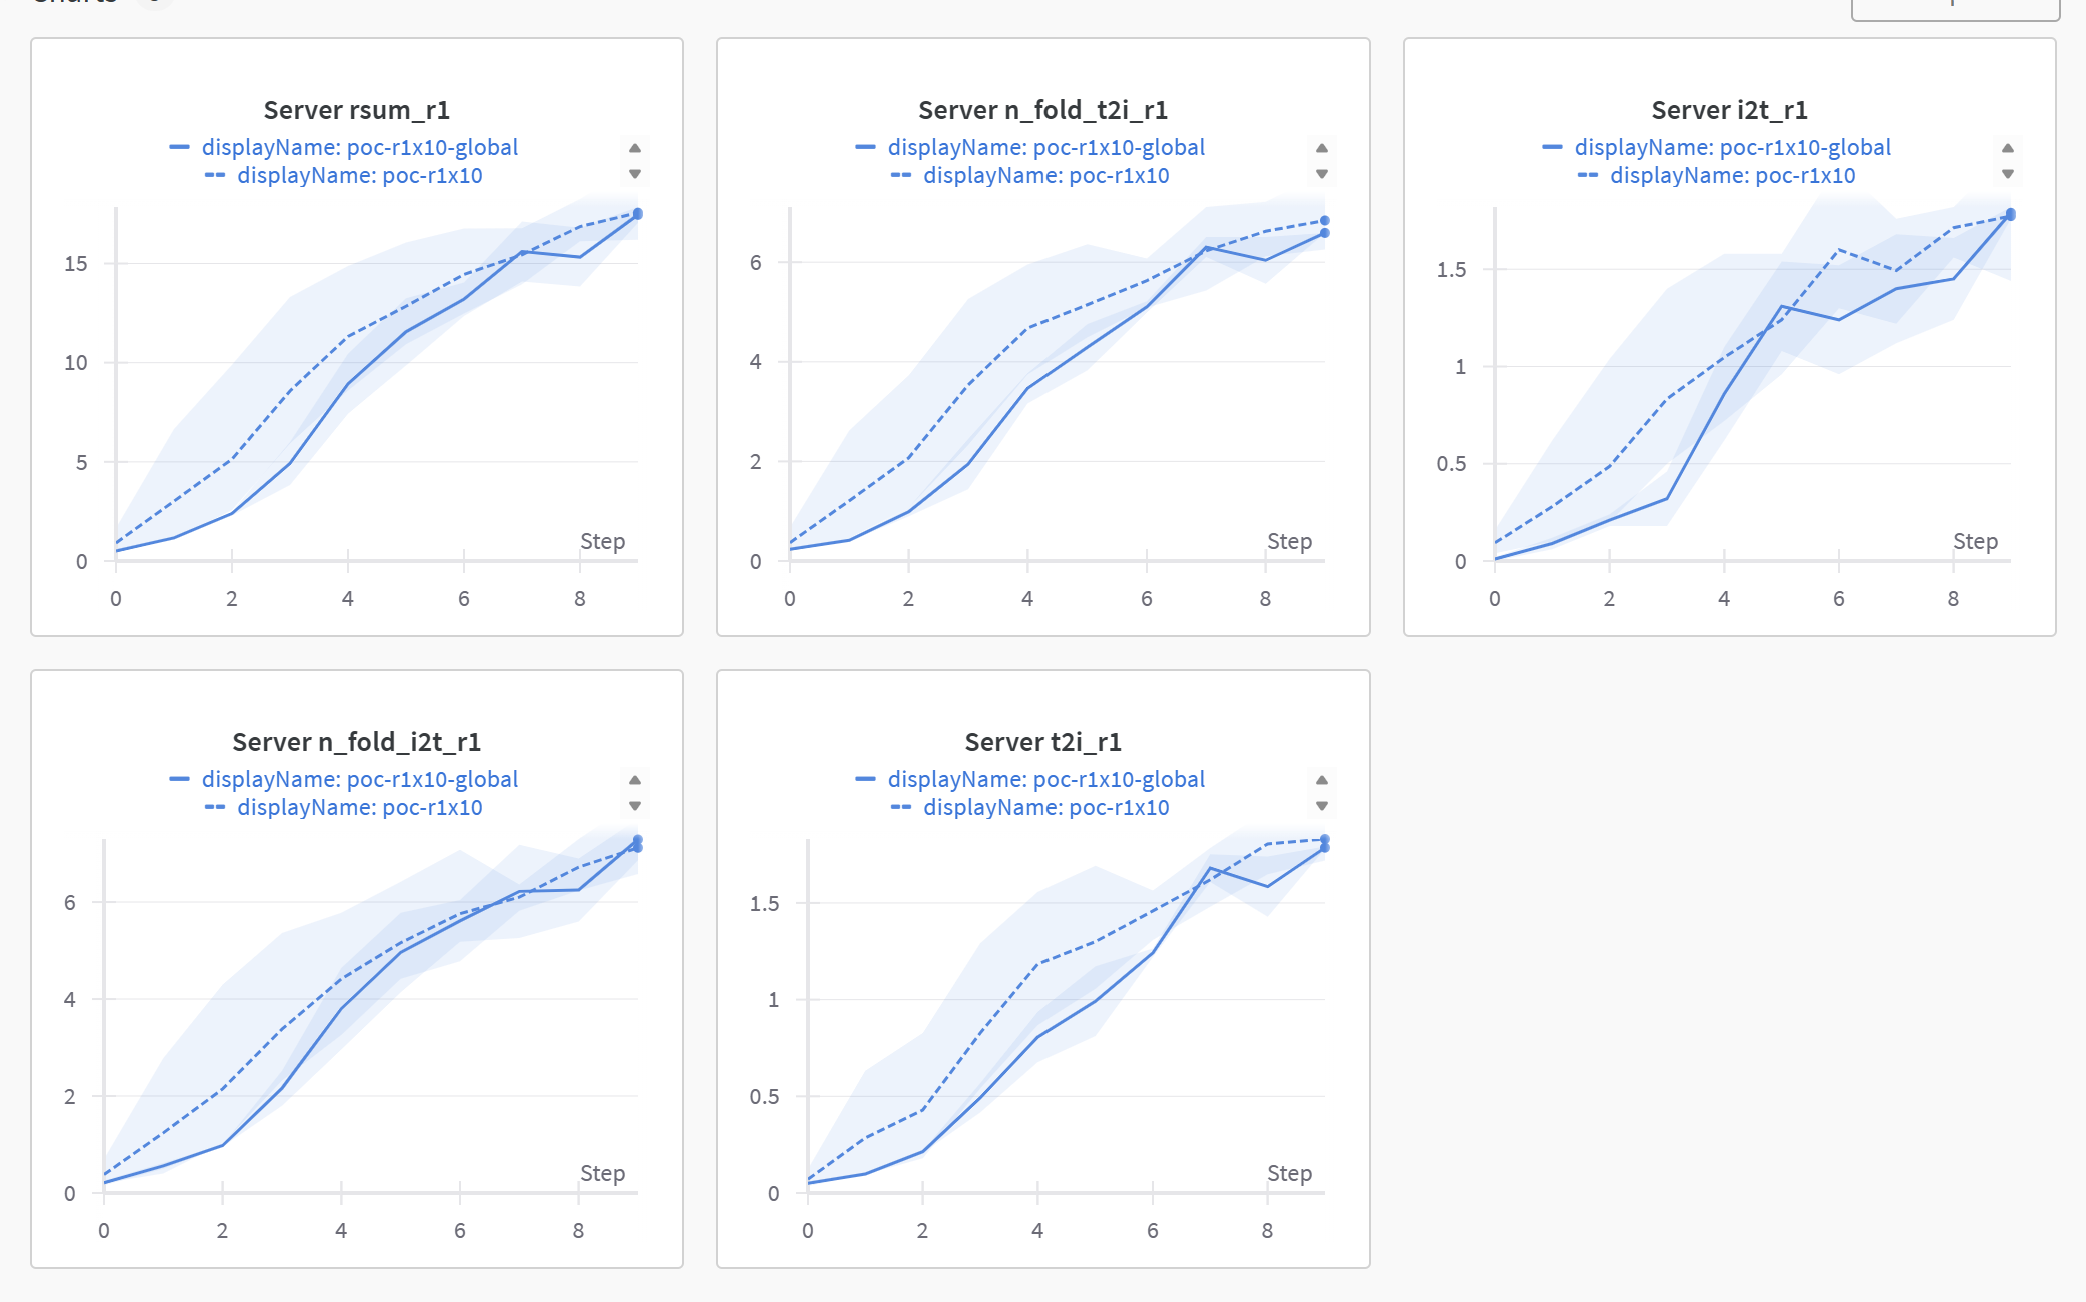
\includegraphics[width=0.8\textwidth]{poc-r1x10.png}
    \caption{Train with 1 client over 10 communication rounds.}
    \label{fig:r1x10}
\end{figure}

In Figure \ref{fig:r1x10}, the parameters used were: 
\begin{lstlisting}
    --contrast_local_inter --contrast_local_intra 
    --interintra_weight 0.5 --max_size 50000 
    --pub_data_num 4000 --feature_dim 64 
    --num_img_clients 0 --num_txt_clients 1 
    --num_mm_clients 0 --client_num_per_round 1 
    --local_epochs 5 --comm_rounds 10 --not_bert 
    --seed 0
\end{lstlisting}
This was run 3 times centralized and 2 times distributed to compare the performance of the two. The end results are shown in Table \ref{table:r1x10}.

\begin{sidewaystable}
    \centering
    \begin{tabular}{|l|l|l|l|l|l|l|l|}
    \hline
    Name & Runtime & ID & i2t\_r1 & n\_fold\_i2t\_r1 & n\_fold\_t2i\_r1 & rsum\_r1 & t2i\_r1 \\
    \hline
    poc-r1x10-global & 5.9h\footnote{computer went to sleep} & 9eebn4qd & 1.82 & 6.86 & 6.588 & 17.06 & 1.792 \\
    poc-r1x10-global & 2.3h & goljw32i & 1.76 & 7.72 & 6.588 & 17.848 & 1.78 \\
    poc-r1x10 & 2.2h & 3u0urus7 & 1.76 & 6.66 & 6.256 & 16.408 & 1.732 \\
    poc-r1x10 & 2.0h & bkiu5ffi & 2.12 & 8.12 & 7.804 & 20.084 & 2.04 \\
    poc-r1x10 & 2.0h & 0g6ia4ds & 1.44 & 6.58 & 6.452 & 16.192 & 1.72 \\
    \hline
    \end{tabular}
    \caption{Comparing the results of centralized vs distributed inference with 1 client over 10 communication rounds.}
    \label{table:r1x10}
\end{sidewaystable}




\section{Future Work}

\section{Conclusion}
% Summarize the findings of the experiment and draw conclusions about the effectiveness of the distributed framework.

\end{document}